\begin{ex}
Uma das principais causas da degradação de peixes frescos é a contaminação por bactérias. O gráfico apresenta resultados de um estudo acerca da temperatura de peixes frescos vendidos em 5 peixarias. O ideal é que esses peixes sejam vendidos com temperaturas entre 2$^{\circ}$ C e 4$^{\circ}$ C.
\begin{center}
  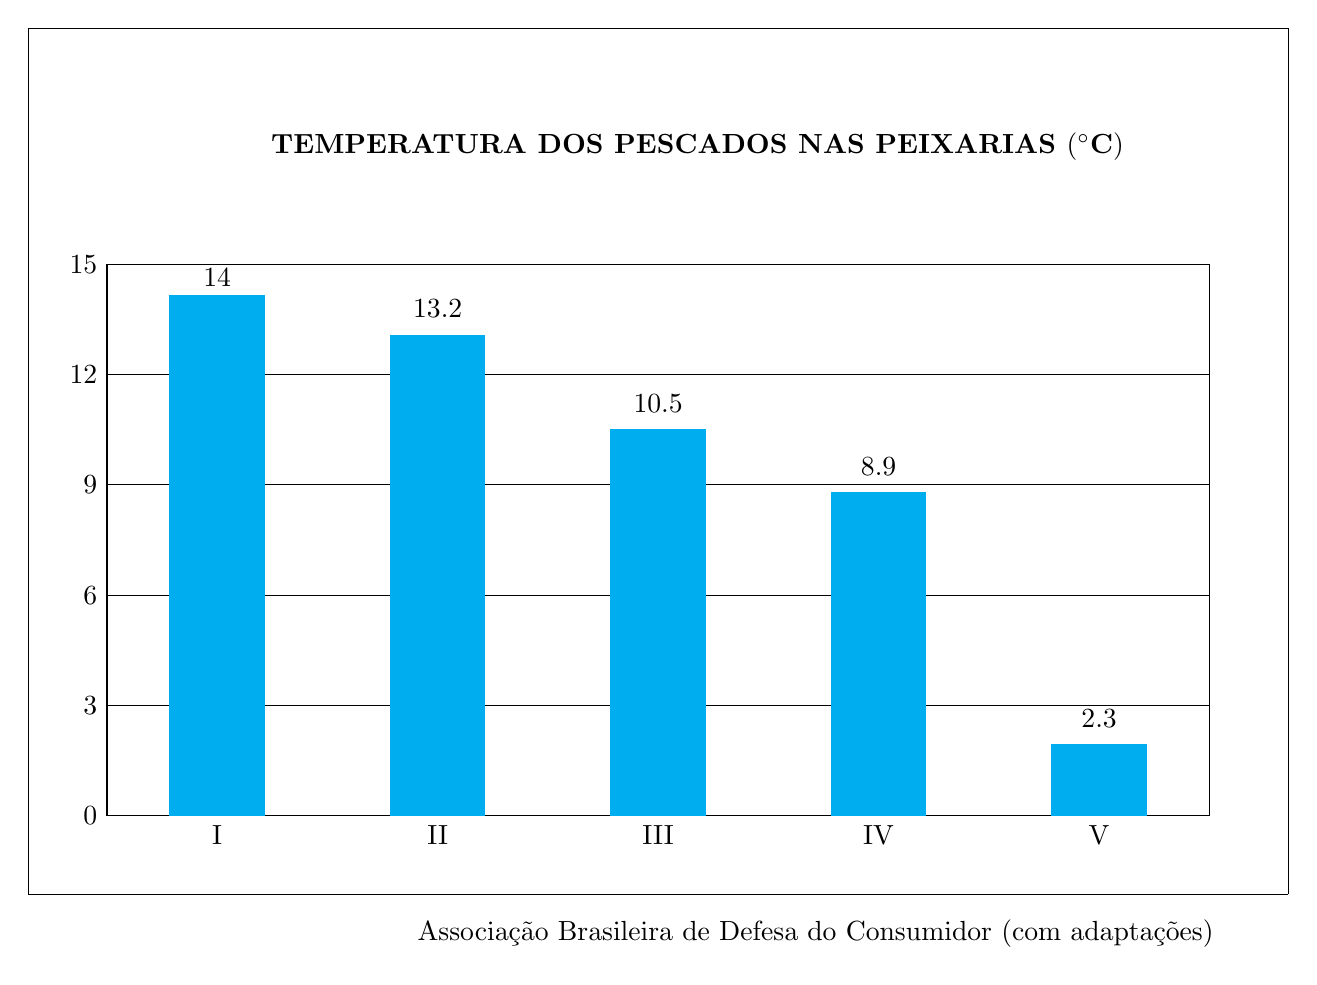
\begin{tikzpicture}
   \draw (0,0)--(14,0);\draw (-1,-1)--(15,-1);\draw (0,1.4)--(14,1.4);
   \draw (0,2.8)--(14,2.8);\draw (0,4.2)--(14,4.2);\draw (0,5.6)--(14,5.6);\draw (0,7)--(14,7);\draw (15,-1)--(15,10);
   \draw (-1,-1)--(-1,10);\draw (-1,10)--(15,10);\draw (0,0)--(0,7);
   \draw (14,0)--(14,7);
   \draw [fill=cyan, draw=cyan] (.8,0)rectangle(2,6.6);\node at (1.4,6.6)  [above]{14};\node at (1.4,0) [below] {I};
   \draw [fill=cyan, draw=cyan] (3.6,0)rectangle(4.8,6.1);\node at (4.2,6.2)[above]{13.2};\node at (4.2,0) [below] {II};
   \draw [fill=cyan, draw=cyan] (6.4,0)rectangle(7.6,4.9);\node at (7,5)  [above]{10.5};\node at (7,0) [below] {III};
   \draw [fill=cyan, draw=cyan] (9.2,0)rectangle(10.4,4.1);\node at (9.8,4.2) [above]{8.9};\node at (9.8,0) [below] {IV};
   \draw [fill=cyan, draw=cyan] (12,0)rectangle(13.2,.9);\node at (12.6,1)  [above]{2.3};\node at (12.6,0) [below] {V}; \node at (0,0) [left] {0}; \node at (0,1.4) [left] {3}; \node at (0,2.8) [left] {6}; \node at (0,4.2) [left] {9}; \node at (0,5.6) [left] {12}; \node at (0,7) [left] {15};
   \draw node at (7.5,8.5)  {\textbf{TEMPERATURA DOS PESCADOS NAS PEIXARIAS $(^{\circ}\textbf{C})$}};
   \draw node at (9,-1.5) {Associação Brasileira de Defesa do Consumidor (com adaptações)};
  \end{tikzpicture}
\end{center}
Selecionando-se aleatoriamente uma das 5 peixarias pesquisadas, a probabilidade de ela vender peixes frescos na condição ideal, é igual a:
   \begin{enumerate}[(a)]
   \item $\frac{1}{2}$
   \item $\frac{1}{3}$
   \item $\frac{1}{4}$
   \item $\frac{1}{5}$
   \item $\frac{1}{6}$
   \end{enumerate}
    \begin{sol}
     resposta: d \\
      uma entre 5 peixarias $\Longrightarrow p=\frac{1}{5}$
    \end{sol}
\end{ex}